
\documentclass[preview,convert,convert={outext=.png,command=\unexpanded{pdftocairo -r 600 -png \infile}}]{standalone}
\usepackage{graphicx}
\usepackage{subfig}
\graphicspath{{/home/ming/academic/tools/latex2word/tests/zh/figures}}

\begin{document}
\thispagestyle{empty}
\begin{figure}[htbp]
    \centering
    \subfloat[]{
        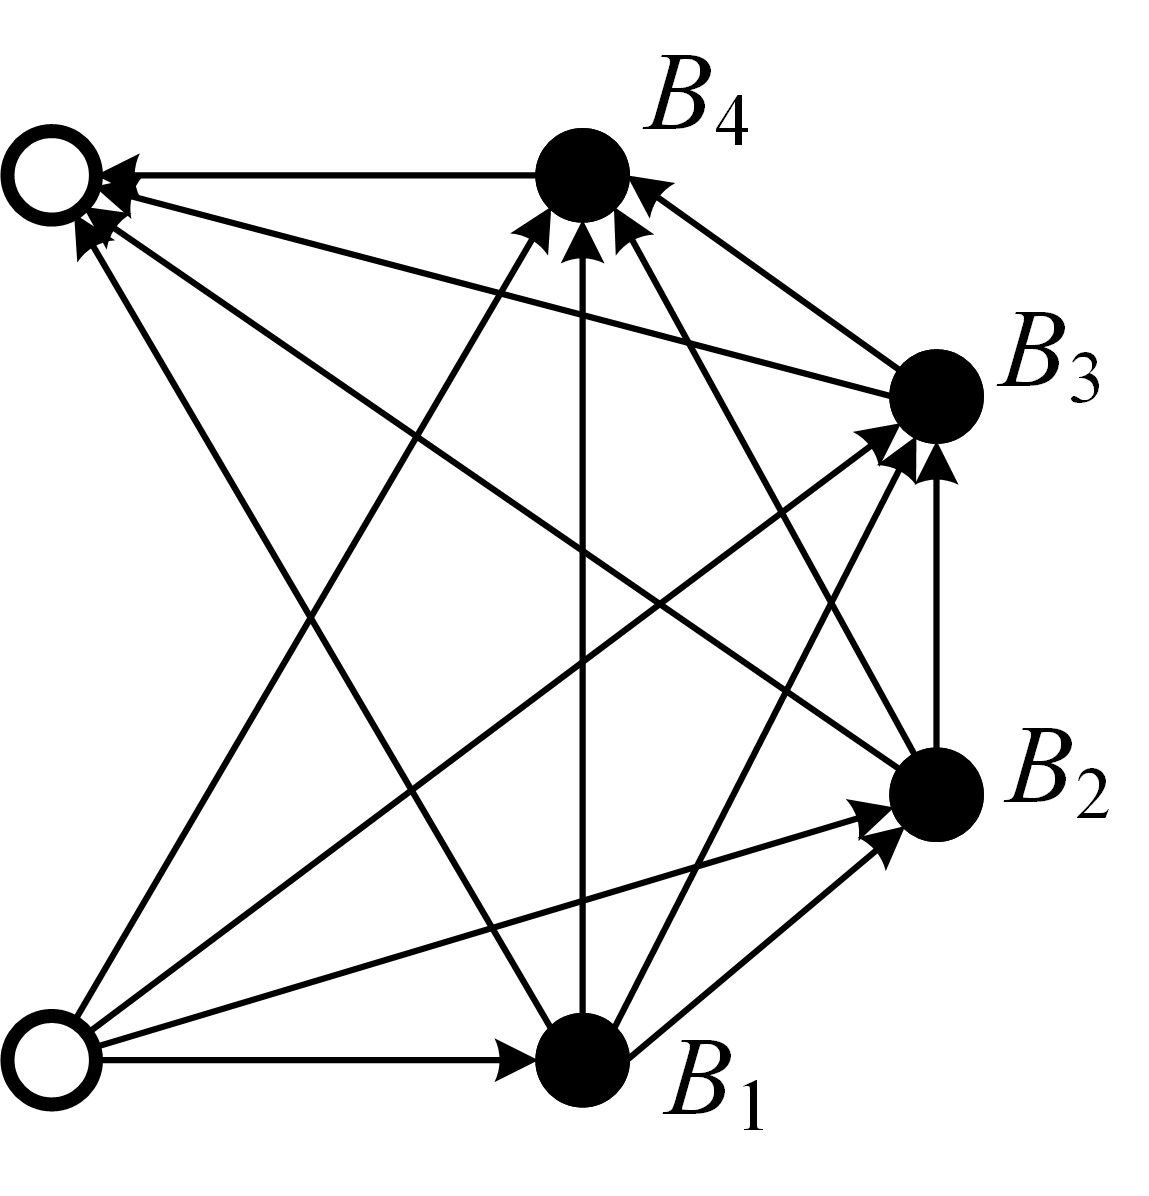
\includegraphics[width=0.31\linewidth]{direct-graph-he.png}
    }
    \subfloat[]{
        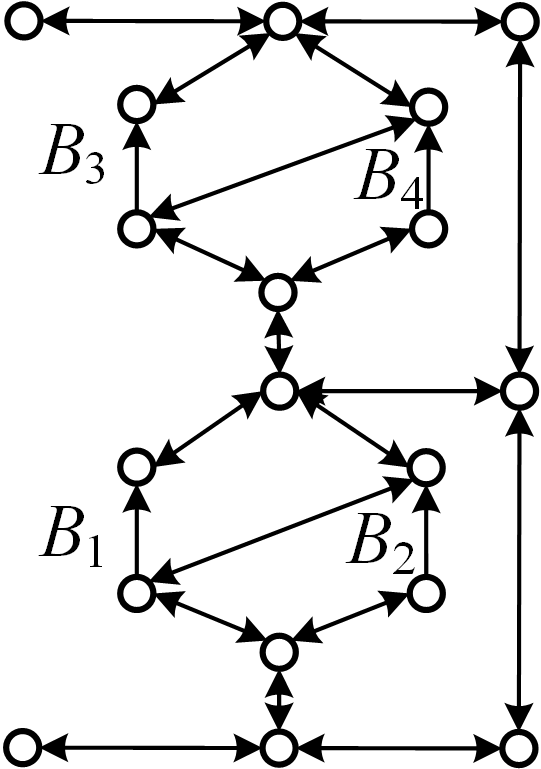
\includegraphics[width=0.23\linewidth]{direct-graph-xu.png}
    }
    \subfloat[]{
        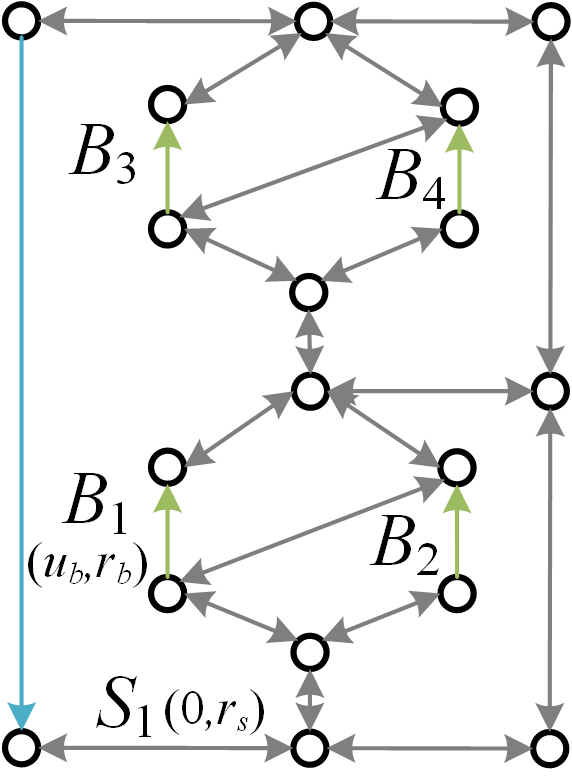
\includegraphics[width=0.24\linewidth]{direct-graph-my.png}
    }
    \\
    \subfloat[]{
        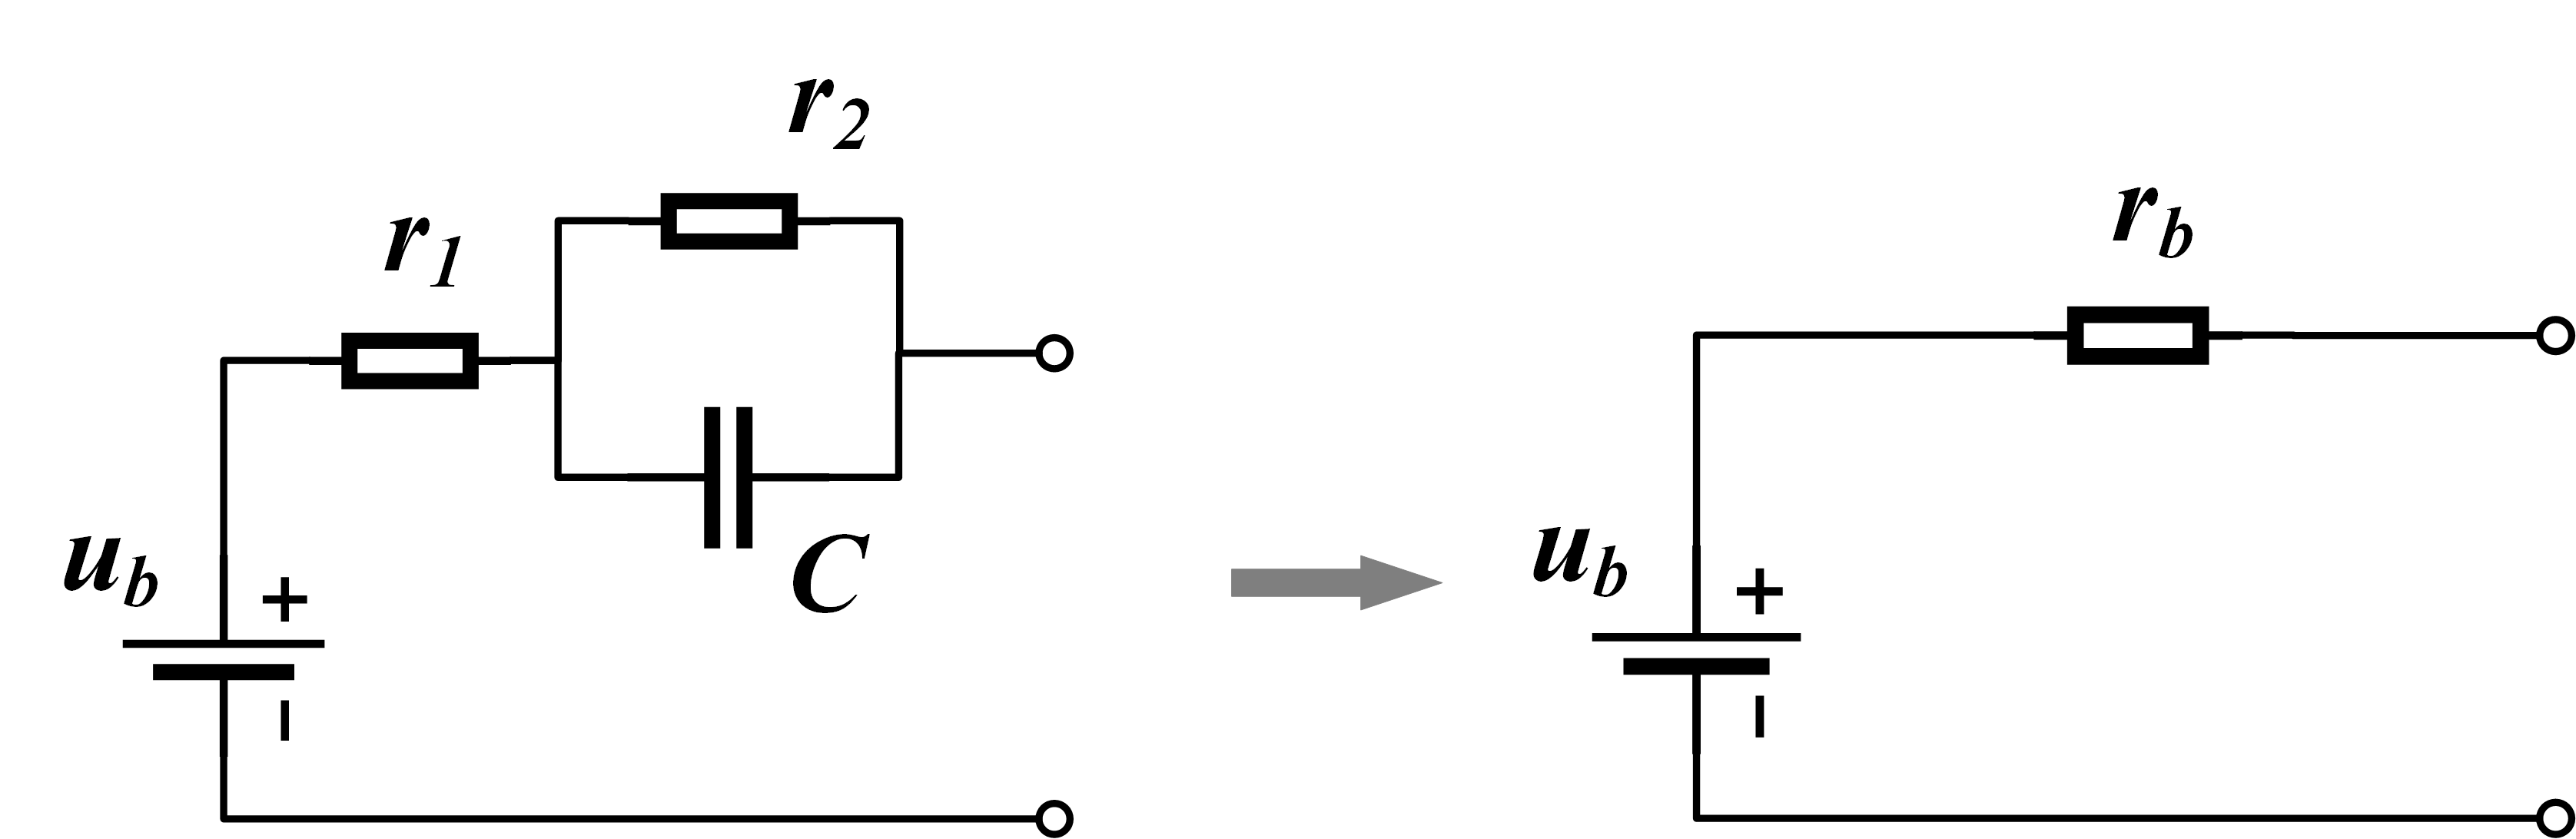
\includegraphics[width=0.8\linewidth]{battery_simple.png}
    }
    % \caption{
%        所使用的有向图模型:(a) He等人的工作 \cite{heExploringAdaptiveReconfiguration2013},(b) 我们之前的工作,(c) 本文改进的模型。(d) 本方法中电池的等效电路。
%    }
    \label{fig:model}
\end{figure}
\end{document}
